\documentclass[tikz,border=2pt]{standalone}
\usepackage{amsmath,amssymb}
\usepackage{tikz}

\begin{document}
% Classical EOQ inventory profile (phone data: y = 22, D = 2 per day): stock jumps to y at
% each instantaneous replenishment and falls linearly to zero in t0 = y/D = 11 days.
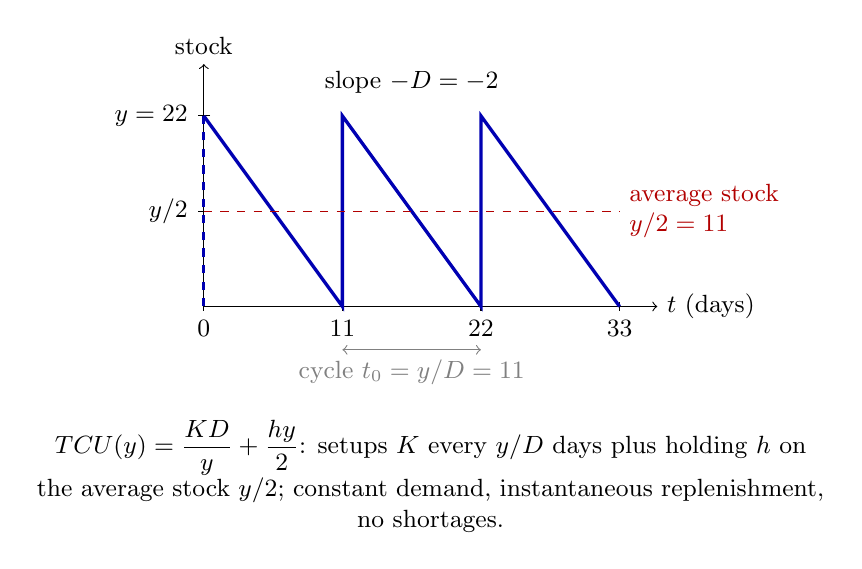
\begin{tikzpicture}[every node/.style={font=\small}, x=0.16cm, y=0.11cm]
	\draw[->] (0,0) -- (36,0) node[right] {$t$ (days)};
	\draw[->] (0,0) -- (0,28) node[above] {stock};
	\foreach \t in {0,11,22,33} {\draw (\t,0.5) -- (\t,-0.5) node[below] {$\t$};}
	\draw (0.5,22) -- (-0.5,22) node[left] {$y=22$};
	\draw (0.5,11) -- (-0.5,11) node[left] {$y/2$};
	\draw[blue!70!black, very thick] (0,22) -- (11,0) -- (11,22) -- (22,0) -- (22,22) -- (33,0);
	\draw[blue!70!black, very thick, dashed] (0,0) -- (0,22);
	\draw[red!70!black, dashed] (0,11) -- (33,11) node[pos=1, right, align=left] {average stock\\ $y/2=11$};
	\draw[<->, gray] (11,-5) -- (22,-5) node[midway, below] {cycle $t_0=y/D=11$};
	\node[anchor=south] at (16.5,23.5) {slope $-D=-2$};
	\node[anchor=north, align=flush center, text width=10cm] at (18,-12) {$TCU(y)=\dfrac{KD}{y}+\dfrac{hy}{2}$: setups $K$ every $y/D$ days plus holding $h$ on the average stock $y/2$; constant demand, instantaneous replenishment, no shortages.};
\end{tikzpicture}
\end{document}
